\documentclass[10pt]{article}   	% use "amsart" instead of "article" for AMSLaTeX format
\usepackage{geometry}                		% See geometry.pdf to learn the layout options. There are lots.
\usepackage[english]{babel}
\geometry{a4paper}                   		% ... or a4paper or a5paper or ... 
%\geometry{landscape}                		% Activate for for rotated page geometry
%\usepackage[parfill]{parskip}    		% Activate to begin paragraphs with an empty line rather than an indent
\usepackage{graphicx}				% Use pdf, png, jpg, or epsß with pdflatex; use eps in DVI mode
\usepackage{fontspec}
\usepackage{multicol}
\setmainfont{Arial}
					
\linespread{1.1}			% TeX will automatically convert eps --> pdf in pdflatex		
\usepackage{amssymb}
\usepackage{eurosym}
\usepackage{colortbl}
\title{MorphicDraw}
\author{Stephan J.C. Eggermont, Sensus}
\begin{document}
\setlength{\parindent}{0pt}
\maketitle
\begin{quote}
\em
MorphicDraw is a drawing application demonstrating some of the power of Morphic.
Morphic is a powerful graphics environment, used in Self, Squeak, Cuis and Pharo.
In an iterative and incremental process we'll build up an application that supports
drawing connected figures.
\end{quote} 

\section{A Morphic Application}
\begin{figure}[htb]
\begin{center}
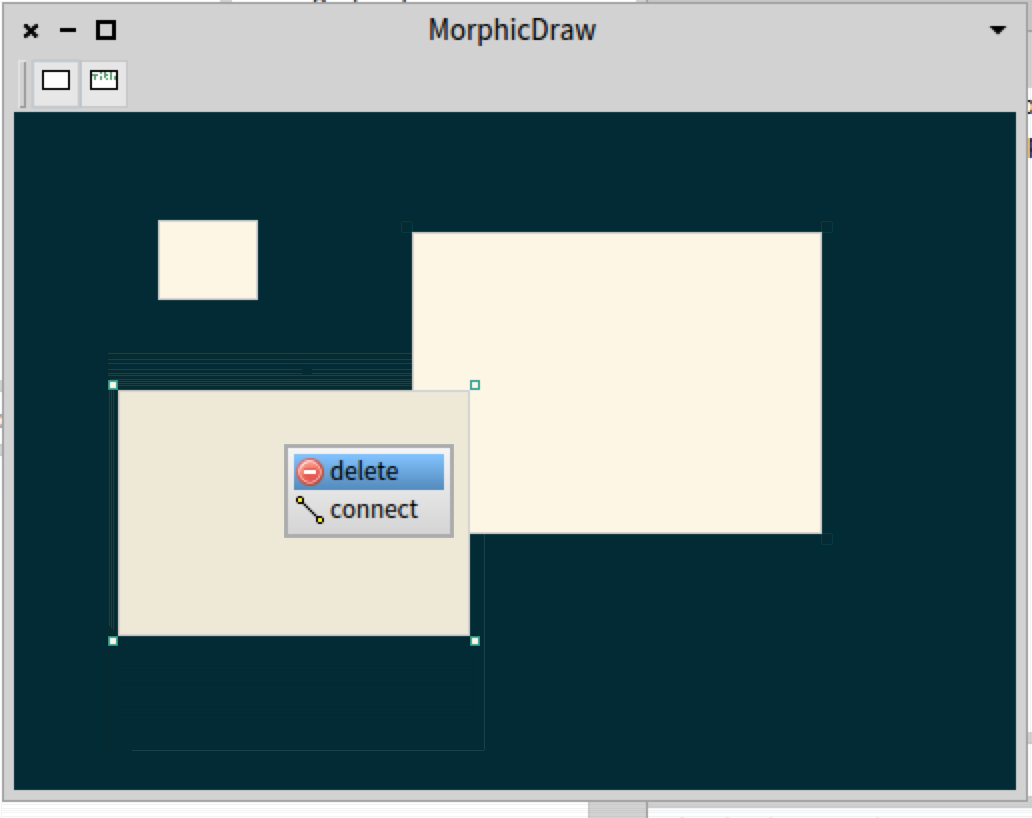
\includegraphics[width=200pt]{SimpleMorphicDrawWindow.png}
\caption{A first iteration of the main window of MorphicDraw}
\label{1stIteration}
\end{center}
\end{figure}
The first iteration (Figure \ref{1stIteration})  shows an application window 
with a toolbar and a drawing area. In the drawing area there are 
three graphical shapes, one of which is selected. A context menu
for the selected shape shows options to delete it and to connect it.

\subsection{An application with a window}
Add a class that represents the application. It has instance variables for 
the different parts. 

\begin{verbatim}
Object subclass: #MorphicDraw
    instanceVariableNames: 'window tools dock'
    classVariableNames: ''
    category: 'MorphicDraw-Model'
\end{verbatim}

Creating a window in Morphic is simple. Open a workspace and DoIt
\begin{verbatim}
StandardWindow new openInWorld 
\end{verbatim} 
This creates a window and opens it on the screen. 
It already has default behaviour for closing and resizing, and a default title. 
All graphical elements in Morphic are subclasses of Morph, and the 
World is a container for all of them. Opening a Morph in the world
positions it and makes it visible. An alternative to opening it directly is
to add it to the (mouse) cursor. In Morphic this is called the hand.
DoIt:
\begin{verbatim}
StandardWindow new openInHand 
\end{verbatim} 
The window is then positioned by clicking.

The MorphicDraw application uses the first, but needs to change 
the window title and default size.

\begin{verbatim}
MorphicDraw>>createWindow
    window := StandardWindow new
        setLabel: 'MorphicDraw';
        extent: 400@400;
        yourself.
\end{verbatim}

StandardWindow is part of PolyMorph. PolyMorph extends Morphic
with theme-ability. PolyMorph widgets often strictly adhere to the theme,
ignoring the Morphic-level setters for colors and borders defined in
their superclassses.  PolyMorph makes the 
Window responsible for adding predefined user interface widgets
to the application Window. For that it uses the TEasilyThemed 
trait. It adds a lot (163 in my current image) of convenience methods.

In Morphic, a toolbar in a window has buttons on it. This iteration of
MorphicDraw uses two buttons to be able to create two different 
graphical shapes.

\begin{verbatim}
MorphicDraw>>createNewCardButton
    ^ window
        newButtonFor: self
        getState: nil
        action: #newCard
        arguments: nil
        getEnabled: nil
        labelForm: MDIcons default cardIcon
        help: 'New Card' translated
\end{verbatim}
The help text is shown when hovering the mouse over the button.
The button is always enabled, and sends the \#newCard message 
without any arguments to self when it is pressed. It has no 
state-dependent behaviour or shape. The icon for the button
is provided by MDIcons default cardIcon (see the Icons section,  p. \pageref{Icons}).

The button for the other shape is similar:
\begin{verbatim}
MorphicDraw>>createNewRectangleButton
    ^ window
        newButtonFor: self
        getState: nil
        action: #newRectangle
        arguments: nil
        getEnabled: nil
        labelForm: MDIcons default rectangleIcon
        help: 'New Rectangle' translated
\end{verbatim}

A toolbar in Morphic consists of two parts, a ToolDockingBar and
a Toolbar. The Toolbar is added to the dock. A DockingBarMorph 
sticks to one edge of the Morph that it is added to.

\begin{verbatim}
MorphicDraw>>createToolBar
    tools := window newToolbar: (Array with: self createNewRectangleButton with: self createNewCardButton).
    dock := window newToolDockingBar.
    dock addMorph: tools
\end{verbatim}

At the class side add a method to open the application

\begin{verbatim}
MorphicDraw>>open
    ^self new open
\end{verbatim}

\section{Icons\label{Icons}}
The current icons in Pharo are bitmap icons. Athens makes it possible
to replace them by SVG, vector based icons. PolyMorph adds the 
ThemeIcons class to make it easy to manage an applications' icons.
In this class a number of utility functions are defined to load and save
icons in png format. 

Create the png icons in an external program
(these were created with Gimp), store them in a directory.
Create a subclass of ThemeIcons
\begin{verbatim}
ThemeIcons subclass: #MDIcons
     instanceVariableNames: ''
    classVariableNames: ''
    category: 'MorphicDraw-Model'
\end{verbatim}
Add two methods containing the names for small- and normal sized icons
\begin{verbatim}
MDIcons>>normalSizeNames
    "Answer the names of the normal icons"
    ^#('rectangle' 'connector' 'card')

MDIcons>>smallSizeNames
    "Answer the names of the small icons. None"
    ^#()
\end{verbatim}
Provide a default instance of this class. At the class side, add 
a class instance variable and a lazy accessor
\begin{verbatim}
MDIcons class
    instanceVariableNames: 'default'

MDIcons class>>default
    ^default ifNil: [ ^self new ]
\end{verbatim}
Now add the icons using a utility method. In a workspace, DoIt
with directory replaced by the fully qualified path name of the
directory containing the icon png files:
\begin{verbatim}
MDIcons default createIconMethodsFromDirectory: directory 
\end{verbatim}
This adds two methods for each png file, one with a base64 encoded
contents and one icon form accessor. Form provides asMorph,
so the icons can be tested by DoIt
\begin{verbatim}
MDIcons default connectorIcon asMorph openInWorld
\end{verbatim}
This opens an ImageMorph with the icon in the World (Fig. \ref{iconhalos}). 
By selecting it with shift-alt, its halos are shown. 
\begin{figure}[htb]
\begin{center}
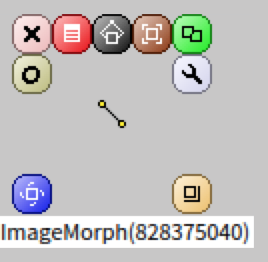
\includegraphics[width=150pt]{ImageIcon.png}
\caption{ImageMorph with icon and halos}
\label{iconhalos}
\end{center}
\end{figure}
With the cross halo the icon can be deleted. 
\section{Shapes and PasteUpMorph}

\section{Toolbar}
\section{Connecting}



\section{Selection and resizing}

\section{Loading the code}
The code can be found on www.smalltalkhub.com, in the repository StephanEggermont/MorphicDraw
Open the Monticello Browser. Add a new repository of type smalltalkhub.com. 
The owner is StephanEggermont, the project is MorphicDraw. User and password are only needed
when you want to commit changes to the repository. Open the repository and load the latest version of
MorphicDraw.

\end{document}  